\chapter{Einleitung}
\label{chapter:Einleitung}

Die Germanedge Solutions GmbH ist Deutschlands Vorreiter in der Digitalisierung der Produktion und
unterstützt Unternehmen mit individuellen Softwarelösungen für die Industrie 4.0 \cite{industry4dot0}.
Darunter auch ein nicht genannter Kunde, welcher Germanedge mit der Optimierung der Planung von Holzpressen beauftragt hat.
Dabei werden Holzbauteile zu Holzbalken verleimt und anschließend in Pressen gepresst.
Die Art und Weise der Anordnung der Bauteile in den Pressen wird als Pressenplan bezeichnet.
Abbildung \ref{figure:pressenplan} visualisiert einen solchen Pressenplan.
Die Presse (grau) presst in Richtung der Pfeile nach unten.
Die Balken (gelb) liegen horizontal und bestehen aus Bauteilen, welche durch die vertikalen (schwarzen) Linien getrennt sind.
Der Rest jedes Balkens ist rot hervorgehoben.

\begin{figure}[h]
    \centering
    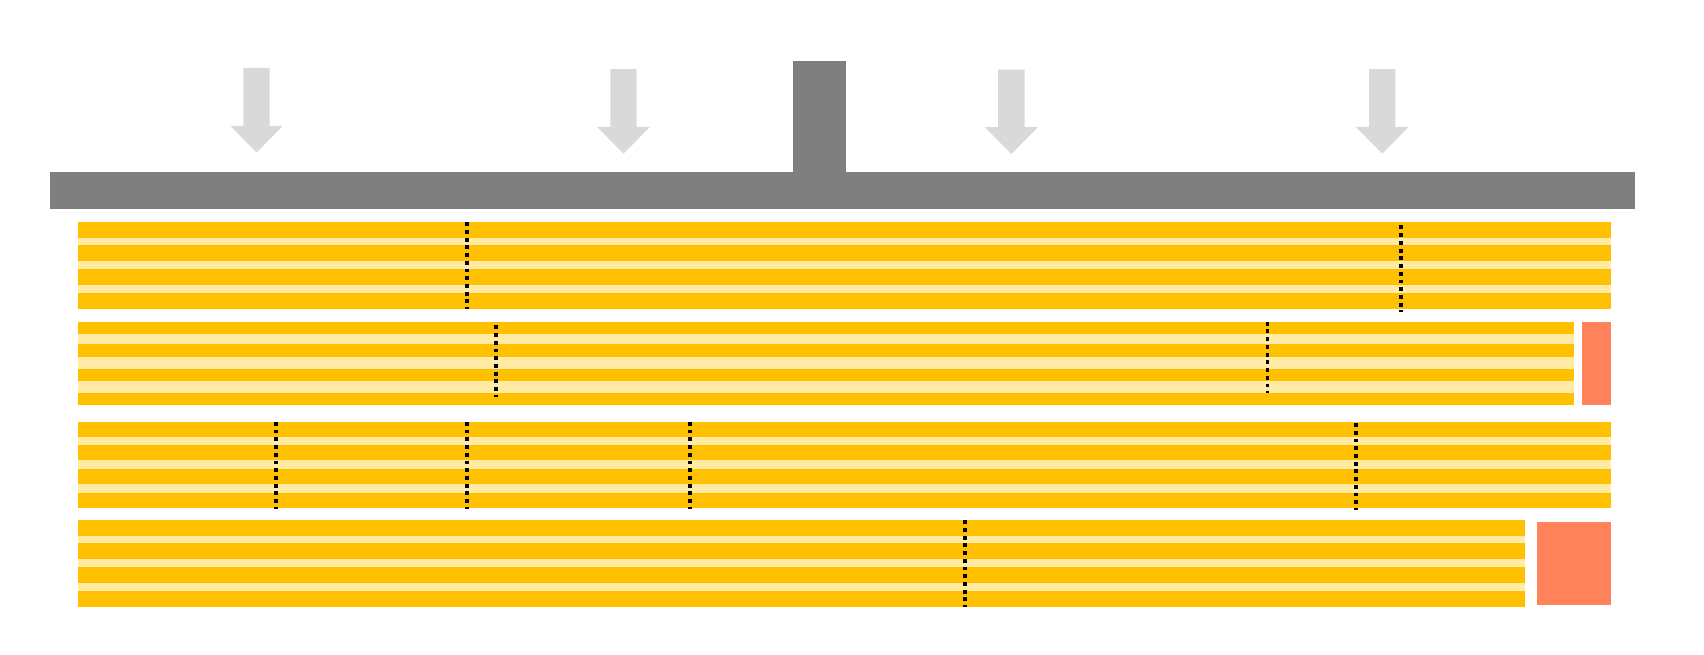
\includegraphics[width=1.00\textwidth, center]{Images/Pressenplan}\\
    \caption{Darstellung eines Pressenplans}
    \label{figure:pressenplan}
\end{figure}

An einen Pressenplan werden verschiedene Anforderungen wie beispielsweise die Gleichheit der Längen aller Balken in einer Presse gestellt.
Neben diesen Anforderungen sind auch einige Optimierungsziele für den Pressenplan von Bedeutung.
Darunter zum Beispiel die Minimierung des Rests, der Balken auf die gleiche Länge auffüllt und somit zusätzliche Materialkosten erzeugt.

Germanedge konnte für dieses Problem bereits eine Lösung finden, diese ist allerdings unter Firmenverschluss.
Es ist lediglich bekannt, dass jene einen heuristischen Ansatz wählt, was bedeutet, dass (optimale) Lösungen verloren gehen.

Daher wird in dieser Arbeit ein neuer, vollständiger Ansatz zur Lösung des Problems gewählt.
Dieser besteht in der Kodierung der Anforderungen an den Pressenplan als Constraints in einem Constraint-System.
Ein Constraint ist eine aussagenlogische Formel, welche unter einer erfüllenden Belegung den Wahrheitswert \texttt{Wahr} haben muss.
Für die dafür in dieser Arbeit verwendeten Satisfiability Modulo Theories (SMT) und deren Sprachstandard SMTLib Version 2.6 \cite{smtlib}
beschreibt folgendes Constraint beispielsweise die Neutralität der Null im Monoid $(\mathbb{N}_0, +, 0)$:

\begin{listing}[H]
    \inputminted{haskell}{Code/Einleitung/MonoidNPlusNull.smt2}
    \caption{SMTLib-Kodierung der Neutralität der Null im Monoid $(\mathbb{N}_0, +, 0)$}
    \label{listing:monoidnnplusnull}
\end{listing}

Ein Constraint-System besteht aus der Konjunktion mehrerer Constraints.
In typischen Anwendungsbereichen von SMT wie der Programmverifikation \cite{smt} werden im Gegensatz zu Beispiel \ref{listing:monoidnnplusnull}
Unbekannte (Variablen) modelliert, für welche der Solver eine erfüllende Belegung unter Beachtung der Constraints ermitteln soll.
So könnte obiges Beispiel als Frage nach dem neutralen Element im Monoid $(\mathbb{N}_0, +, x)$ folgend formuliert werden:

\begin{listing}[H]
    \inputminted{haskell}{Code/Einleitung/MonoidNPlusZ.smt2}
    \caption{SMTLib-Kodierung des unbekannten neutralen Elements $x$ im Monoid $(\mathbb{N}_0, +, x)$}
    \label{listing:monoidnnplusz}
\end{listing}

Um zum Pressenplanungsproblem zurückzukehren, stellt sich die Frage, wie dieses in SMTLib Version 2.6 kodiert werden kann.
Eine Beispieleingabe von Bauteilen könnte folgende sein:

\begin{table}[H]
    \centering
    \begin{tabular}{|c|c|c|}
        \hline
        \textbf{Länge} & \textbf{Höhe} & \textbf{Anzahl} \\
        \hline
        5345.0 & 235.0 & 4 \\
        5219.0 & 287.0 & 40 \\
        5319.0 & 287.0 & 36 \\
        5220.0 & 235.0 & 59 \\
        4796.0 & 287.0 & 13 \\
        5320.0 & 194.0 & 48 \\
        4740.0 & 287.0 & 34 \\
        \hline
    \end{tabular}
    \caption{Beispieleingabe von Bauteilen, jede Zeile entpricht einer Bauteilspezifikation}
    \label{table:bauteileingabe}
\end{table}

Da das Formulieren der Constraints für einen Pressenplan mit gegebenen Bauteilen händisch in der Constraint-Sprache SMTLib sehr schwer- und fehleranfällig ist,
erzeugt ein Programm in einer Gastsprache das Constraint-System für die Constraint-Sprache.
Für diese Arbeit wird als jene Gastsprache Haskell \cite{haskellhistory} gewählt.
Mit der Haskell-Bibliothek \texttt{Hasmtlib} \cite{hasmtlib} lässt sich beispielhaft das bereits erwähnte Constraint gleicher Länge aller Balken in einer Presse folgend formulieren:

\begin{listing}[H]
    \inputminted{haskell}{Code/Einleitung/PressenlängeConstraintHaskell.hs}
    \caption{Haskell-Code für das Constraint gleicher Länge aller Balken einer Presse}
    \label{listing:barLengthCode}
\end{listing}

Die Bibliothek erzeugt dann das Constraint-System in der Constraint-Sprache SMTLib.
Folgend ein beliebiger Ausschnitt der SMTLib-Kodierung:

\begin{listing}[H]
    \inputminted{bash}{Code/Einleitung/PressenlängeConstraintSMTLib.smt2}
    \caption{Ausschnitt der Kodierung eines Pressenplanungsproblems}
    \label{listing:barLengthSMTlib}
\end{listing}

Die Kodierung wird an einen SMT-Solver gegeben, welcher die Erfüllbarkeit des Problems bestimmt und für den Fall \textit{erfüllbar} eine erfüllende Belegung für die Variablen des Problems ermittelt.
Zum Beispiel:

\begin{listing}[H]
    \inputminted{bash}{Code/Einleitung/PressenlängeConstraintSolverOutput.smt2}
    \caption{Ausschnitt des Solver-Outputs der Lösung eines Pressenplanungsproblems}
    \label{listing:barLengthSolverOutput}
\end{listing}

Jene Belegung transformiert das Programm dann in das gewünschte Ausgabeformat:

\begin{table}[H]
    \centering
    \begin{tabular}{|c|c|c|c|c|}
        \hline
        \textbf{Presse} & \textbf{Schicht} & \textbf{Position} & \textbf{Länge} & \textbf{Höhe} \\
        \hline
        1 & 1 & 1 & 5345.0 & 235.0 \\
        1 & 1 & 2 & 5345.0 & 235.0 \\
        1 & 1 & 3 & 5345.0 & 235.0 \\
        1 & 2 & 1 & 5219.0 & 287.0 \\
        \ldots & \ldots & \ldots & \ldots & \ldots \\
        \hline
    \end{tabular}
    \caption{Beispielausgabe des Pressenplans}
    \label{table:pressenplan}
\end{table}

Die Struktur dieser Arbeit ist folgende:

In Kapitel \ref{chapter:fol} werden die, für das weitere Verständnis der Arbeit erforderlichen, Grundlagen der Prädikatenlogik erklärt.

Danach wird in Kapitel \ref{chapter:problem} das Problem der Pressenplanung dargelegt, modelliert und nach, für das Problem relevanten, Zielfunktionen optimiert.

Folgend wird in Kapitel \ref{chapter:smt} gezeigt, wie Erfüllbarkeitsprobleme der Satisfiability Modulo Theories im Sprachstandard SMTLib Version 2.6 kodiert werden können.

In Kapitel \ref{chapter:implementierung} wird zunächst auf wenige, notwendige Grundlagen von Haskell eingegangen,
bevor die Kodierung der in Abschnitt \ref{section:modellierung} erstellten Modelle des Pressenplanungsproblems in Haskell erläutert wird.
Zusätzlich werden dort einige Erweiterungen der Haskell-Bibliothek \texttt{Hasmtlib} diskutiert.

Weiter werden die Ergebnisse der Kodierungen in Kapitel \ref{chapter:auswertung} mithilfe von Laufzeitmessungen ausgewertet.

Abschließend wird das Ergebnis dieser Arbeit in Kapitel \ref{chapter:zusammenfassung} zusammengefasst.